%%%%%%%%%%%%%%%%%%% EJERCICIO 2 %%%%%%
%%%%%%%%%%%%%%%%%%% EJERCICIO 2a %%%%%%
\textbf{Ejemplo 2 }\\
Una deuda de  600.000 COP se va a cancelar en 7 pagos trimestrales con un interés del 9\% periódo trimestre vencido. Si al momento de efectuar el pago número 3 se efectúa un abono 2 extraordinario, no pactado, de 250.000 COP. Se pide: 
a) Elaborar una tabla de amortización sin considerar el abono.\\
b) Elaborar una tabla suponiendo que la cuota extra se abona a capital sin reliquidar la cuota. \\
c) Elaborar una tabla de amortización si al hacer el abono extra se pide reliquidar la cuota.\\

%\newpage %USAR SOLO SI EL SOLUCIÓN QUEDA SOLO Y ES NECESARIO BAJARLO A LA SIGUIENTE PAGINA
\textbf{Solución.}\\
%La tabla ira centrada
\begin{center}
	\renewcommand{\arraystretch}{1.5}% Margenes de las celdas
	%Creación de la cuadricula de 3 columnas
	\begin{longtable}[H]{|c|c|c|}
		%Creamos una linea horizontal
		\hline
		%Definimos el color de la primera fila
		\rowcolor[HTML]{FFB183}
		%%%%% INICIO ASIGNACIÓN PERIODO FOCAL %%%%%%%
		%%%%%%%%%% INICIO TITULO
		%Lo que se hace aquí es mezclar las 3 columnas en una sola
		\multicolumn{3}{|c|}{\cellcolor[HTML]{FFB183}\textbf{1. Asignación período focal}}  \\ \hline
		\multicolumn{3}{|c|}{$pf = \textit{0 ptv}$}   \\\hline
		%%%%%%%%%% FIN TITULO
		%%%%% INICIO DECLARACIÓN DE VARIABLES %%%%%%%
		%%%%%%%%%% INICIO TITULO
		%Lo que se hace aquí es mezclar las 3 columnas en una sola
		\multicolumn{3}{|c|}{\cellcolor[HTML]{FFB183}\textbf{2. Declaración de variables}}   \\ \hline
		%%%%%%%%%% FIN TITULO
		%%%%%%%%%% INICIO DE MATEMÁTICAS
		%Cada & hace referencia al paso de la siguiente columna
		\multicolumn{2}{|c|}{$\hspace{2 cm}VP= 600.000 \ COP\hspace{2 cm}$} & $i \equiv 9\% \textit{ ptv}$ \\
		\multicolumn{2}{|c|}{$\hspace{2 cm}n_1=7 \textit{ ptv} \hspace{2 cm}$} & $\hspace{2 cm}R = ? COP  \hspace{2 cm}$ \\ \hline
		
		
		
		%%%%%%%%%% FIN DE MATEMÁTICAS
		%%%%% FIN DECLARACIÓN DE VARIABLES
		
		
		%%%%% INICIO FLUJO DE CAJA
		\rowcolor[HTML]{FFB183}
		\multicolumn{3}{|c|}{\cellcolor[HTML]{FFB183}\textbf{3. Diagrama de flujo de caja}} \\ \hline
		%Mezclamos 3 columnas y pondremos el dibujo
		%%%%%%%%%%%%% INSERCIÓN DE LA IMAGEN
		%Deberán descargar las imágenes respectivas del drive y pegarlas en la carpeta
		%n_capitulo/img/ejemplos/1/capitulo1ejemplo1.pdf  (el /1/ es el numero del ejemplo)
		\multicolumn{3}{|c|}{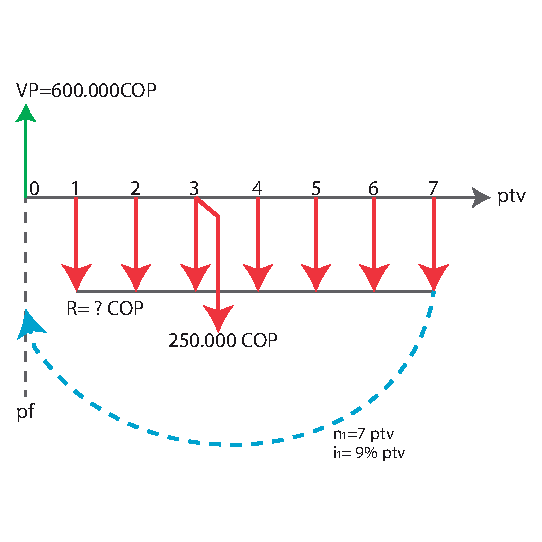
\includegraphics[trim=-78 -5 -78 -5]{7_Capitulo/img/ejemplos/2/Capitulo7Ejercicio2.pdf} }
		
		
		\\ \hline
		%%%%%%%%%%%%% FIN INSERCIÓN DE IMAGEN
		%%%%%FIN FLUJO DE CAJA
		
		
		
		%%%%% INICIO DECLARACIÓN FORMULAS
		%%%%%%%%%%% INICIO TITULO
		\rowcolor[HTML]{FFB183}
		\multicolumn{3}{|c|}{\cellcolor[HTML]{FFB183}\textbf{4. Declaración de fórmulas}}    \\ \hline
		%%%%%%%%%%% FIN TITULO
		%%%%%%%%%%% INICIO MATEMÁTICAS
		\multicolumn{3}{|c|}{$VP=R(\frac{1-(1+i)^{-n}}{i}) \hspace{0.4 cm} \textit{Valor presente de una serie uniforme vencida}$} \\ \hline
		
		%%%%%%%%%% FIN MATEMÁTICAS
		%%%%%% INICIO DESARROLLO MATEMÁTICO
		\rowcolor[HTML]{FFB183}
		%%%%%%%%%%INICIO TITULO
		\multicolumn{3}{|c|}{\cellcolor[HTML]{FFB183}\textbf{5. Desarrollo matemático}}       \\ \hline
		%%%%%%%%%% FIN TITULO
		%%%%%%%%%% INICIO MATEMÁTICAS
		\multicolumn{3}{|c|}{$ 600.000 \ COP =R(\frac{1-(1+0.09)^{-7}}{0.09})\hspace{0.2 cm}\rightarrow \hspace{0.2 cm}R= 119.214,31 \ COP$} \\ \hline
		
		%%%%%%%%%% FIN MATEMÁTICAS
		%%%%%% FIN DESARROLLO MATEMÁTICO
		%%%%%% INICIO RESPUESTA
		\rowcolor[HTML]{FFB183}
		%%%%%%%%%%INICIO TITULO
		\multicolumn{3}{|c|}{\cellcolor[HTML]{FFB183}\textbf{6. Respuesta}}   \\ \hline
		%%%%%%%%%% FIN TITULO
		%%%%%%%%%% INICIO RESPUESTA MATEMÁTICA
		\multicolumn{3}{|c|}{$\mathbf{R= 119.214,31 \ COP}$}
		\begin{comment}
		\multicolumn{3}{|p{\textwidth}|}{
		$F_{4} = F_{5} = 21.609,84 \ COP$ .}
		\end{comment} 
		\\ \hline
		%%%%%%%%%% FIN MATEMÁTICAS
		%%%%%% FIN RESPUESTA
	\end{longtable}
	%Se crean dos lineas en blanco para que no quede el siguiente texto tan pegado
	%\newline \newline %USARLO SI CREES QUE ES NECESARIO
\end{center}
%%%%%%%%%%%%%%%%%%%%%%%%%%FIN EJERCICIO 2a %%%%%%%%%%%%%%%%%%%%%%%%%%%
\newpage
Ahora elaboramos la tabla sin tener en cuenta ninguna cuota extra ya que no se han pactado.

\begin{spacing}{1.1}
	\begin{center}
		\begin{tabular}{|p{1cm}|p{2cm}|p{2cm}|p{2cm}|p{3cm}|}
			\hline
			\textbf{PER\ (1)} & \textbf{SALDO DEUDA (2)=(2)-(5)} & \textbf{INTERESES  (3)=(2)(i)} & \textbf{PAGO\ (4)= COP  R- COP  L } & \textbf{AMORTIZACIÓN  (5)=(4)-(3)} \\ \hline
			
			0                 &   600.000 \ COP                     & ---------                       & ---------                   & ---------                          \\ \hline
			1                 &   534.785,69 \ COP                     &  54.000,00 \ COP                    &  119.214,31 \ COP                &  65.214,31 \ COP                        \\ \hline
			2                 &  463.702,09 \ COP                     &  48.130,71 \ COP                    &  119.214,31 \ COP                &    71.083,60 \ COP                        \\ \hline
			3                 &  386.220,97 \ COP                     &  41.733,19 \ COP                     &  119.214,31 \ COP                &   77.481,12 \ COP                        \\ \hline
			4                 &  301.766,55 \ COP                     &  34.759,88 \ COP                     &  119.214,31 \ COP                &  84.454,42 \ COP                        \\ \hline
			5                 &  209.711,23 \ COP                     &  27.158,99 \ COP                     &  119.214,31 \ COP                &   92.055,32 \ COP                        \\ \hline
			6                 &  109.370,93 \ COP                     &  18.874,01 \ COP                     &  119.214,31 \ COP                &  100.340,30 \ COP                       \\ \hline
			7                 &  0,00 \ COP                           &  9.843,38 \ COP                      &  119.214,31 \ COP                &  109.370,93 \ COP                       \\ \hline
		\end{tabular}
	\end{center}
\end{spacing}

La primera forma se puede presentar cuando, al cancelar la tercera cuota, el deudor decide efectuar un abono de    250.000 \ COP, adicional a su cuota ordinaria periódica, entonces la tabla quedará así:
\begin{spacing}{1.1}
	\begin{center}
		\begin{tabular}{|p{1cm}|p{2cm}|p{2cm}|p{2cm}|p{3cm}|}
			\hline
			\textbf{PER\ (1)} & \textbf{SALDO DEUDA (2)=(2)-(5)} & \textbf{INTERESES  (3)=(2)(i)} & \textbf{PAGO\ (4)= COP  R- COP  L } & \textbf{AMORTIZACIÓN  (5)=(4)-(3)} \\ \hline
			
			0                 &  600.000,00 \ COP                     & ---------                       & ---------                   & ---------                          \\ \hline
			1                 &  534.785,69 \ COP                     &  54.000,00 \ COP                    &  119.214,31 \ COP                &  65.214,31 \ COP                        \\ \hline
			2                 &  463.702,09 \ COP                     &  48.130,71 \ COP                    &  119.214,31 \ COP                &  71.083,60 \ COP                        \\ \hline
			3                 &  136.220,97 \ COP                     &  41.733,19 \ COP                     &  369.214,31 \ COP                &  327.481,12 \ COP                       \\ \hline
			4                 &  29.266,55 \ COP                      &  12.259,89 \ COP                     &  119.214,31 \ COP                &  106.954,42 \ COP                       \\ \hline
			5                 &  0,00 \ COP                           &  2.633,99 \ COP                      &  31.900,54 \ COP                 &  29.266,55 \ COP                        \\ \hline
		\end{tabular}
	\end{center}
\end{spacing}

El pago del período 5 debe ser igual a los intereses más el saldo de la deuda, esto es:
\begin{center}
	 2.633,99 \ COP +  29.266,55 \ COP=  31.900,40 \ COP
\end{center}
Obsérvese que la deuda se canceló antes de lo previsto.\\

%%%%%%%%%%%%%%%%%%% EJERCICIO 2b %%%%%%
La segunda forma se puede presentar cuando, al momento de efectuar el pago de la tercera cuota, el deudor desea hacer un abono extra de  250.000 COP, pero exige reliquidación de la cuota para conservar el plazo originalmente pactado, entonces el capital insoluto o saldo de la deuda del período 3 deberá ser cancelada en los 4 períodos restantes, por tanto la nueva cuota será:\\

%\newpage %USAR SOLO SI EL SOLUCIÓN QUEDA SOLO Y ES NECESARIO BAJARLO A LA SIGUIENTE PAGINA
\textbf{Solución.}
%La tabla ira centrada
\begin{center}
	\renewcommand{\arraystretch}{1.5}% Margenes de las celdas
	%Creación de la cuadricula de 3 columnas
	\begin{longtable}[H]{|c|c|c|}
		%Creamos una linea horizontal
		\hline
		%Definimos el color de la primera fila
		\rowcolor[HTML]{FFB183}
		%%%%% INICIO ASIGNACIÓN PERIODO FOCAL %%%%%%%
		%%%%%%%%%% INICIO TITULO
		%Lo que se hace aquí es mezclar las 3 columnas en una sola
		\multicolumn{3}{|c|}{\cellcolor[HTML]{FFB183}\textbf{1. Asignación período focal}}  \\ \hline
		\multicolumn{3}{|c|}{$pf = \textit{0 ptv}$}   \\\hline
		%%%%%%%%%% FIN TITULO
		%%%%% INICIO DECLARACIÓN DE VARIABLES %%%%%%%
		%%%%%%%%%% INICIO TITULO
		%Lo que se hace aquí es mezclar las 3 columnas en una sola
		\multicolumn{3}{|c|}{\cellcolor[HTML]{FFB183}\textbf{2. Declaración de variables}}   \\ \hline
		%%%%%%%%%% FIN TITULO
		%%%%%%%%%% INICIO DE MATEMÁTICAS
		%Cada & hace referencia al paso de la siguiente columna
		\multicolumn{2}{|c|}{$\hspace{2 cm}VP=  136.220,97 \ COP \hspace{2 cm}$} & $i \equiv 9\% \textit{ ptv}$ \\
		\multicolumn{2}{|c|}{$\hspace{2 cm}n_2=4 \textit{ ptv} \hspace{2 cm}$} & $\hspace{2 cm}R = ? COP  \hspace{2 cm}$ \\ \hline
		
		
		
		%%%%%%%%%% FIN DE MATEMÁTICAS
		%%%%% FIN DECLARACIÓN DE VARIABLES
		
		
		%%%%% INICIO FLUJO DE CAJA
		\rowcolor[HTML]{FFB183}
		\multicolumn{3}{|c|}{\cellcolor[HTML]{FFB183}\textbf{3. Diagrama de flujo de caja}} \\ \hline
		%Mezclamos 3 columnas y pondremos el dibujo
		%%%%%%%%%%%%% INSERCIÓN DE LA IMAGEN
		%Deberán descargar las imágenes respectivas del drive y pegarlas en la carpeta
		%n_capitulo/img/ejemplos/1/capitulo1ejemplo1.pdf  (el /1/ es el numero del ejemplo)
		\multicolumn{3}{|c|}{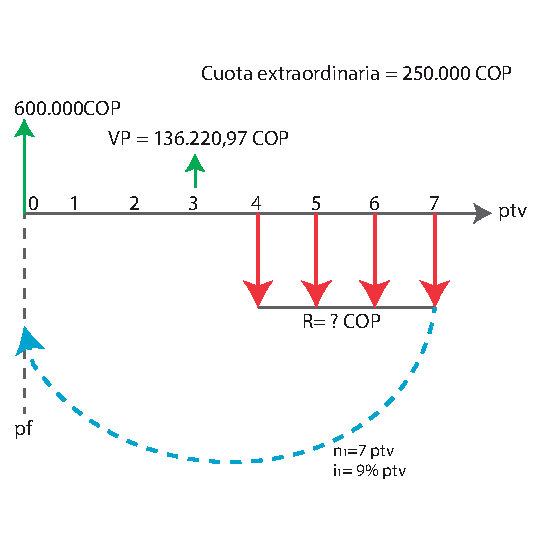
\includegraphics[trim=-78 -5 -78 -5]{7_Capitulo/img/ejemplos/2/Capitulo7Ejercicio2b.pdf} }
		
		
		\\ \hline
		%%%%%%%%%%%%% FIN INSERCIÓN DE IMAGEN
		%%%%%FIN FLUJO DE CAJA
		
		
		
		%%%%% INICIO DECLARACIÓN FORMULAS
		%%%%%%%%%%% INICIO TITULO
		\rowcolor[HTML]{FFB183}
		\multicolumn{3}{|c|}{\cellcolor[HTML]{FFB183}\textbf{4. Declaración de fórmulas}}    \\ \hline
		%%%%%%%%%%% FIN TITULO
		%%%%%%%%%%% INICIO MATEMÁTICAS
		\multicolumn{3}{|c|}{$VP=R(\frac{1-(1+i)^{-n}}{i}) \hspace{0.4 cm} \textit{Valor presente de una serie uniforme}$} \\ \hline
		
		%%%%%%%%%% FIN MATEMÁTICAS
		%%%%%% INICIO DESARROLLO MATEMÁTICO
		\rowcolor[HTML]{FFB183}
		%%%%%%%%%%INICIO TITULO
		\multicolumn{3}{|c|}{\cellcolor[HTML]{FFB183}\textbf{5. Desarrollo matemático}}       \\ \hline
		%%%%%%%%%% FIN TITULO
		%%%%%%%%%% INICIO MATEMÁTICAS
		\multicolumn{3}{|p{\textwidth}|}{Después del abono extraordinario de 250.000 COP el saldo de la deuda es ahora de 136.220,97 COP que se tomará como nuevo capital inicial, por lo tanto:} \\
		\multicolumn{3}{|c|}{$ 136.220 \ COP =R(\frac{1-(1+0.09)^{-4}}{0.09})\hspace{0.2 cm}\rightarrow \hspace{0.2 cm}R= 42.047,14 \ COP$} \\ \hline
		
		%%%%%%%%%% FIN MATEMÁTICAS
		%%%%%% FIN DESARROLLO MATEMÁTICO
		%%%%%% INICIO RESPUESTA
		\rowcolor[HTML]{FFB183}
		%%%%%%%%%%INICIO TITULO
		\multicolumn{3}{|c|}{\cellcolor[HTML]{FFB183}\textbf{6. Respuesta}}   \\ \hline
		%%%%%%%%%% FIN TITULO
		%%%%%%%%%% INICIO RESPUESTA MATEMÁTICA
		\multicolumn{3}{|c|}{$\mathbf{R = 42.047,14  \ COP}$}
		\begin{comment}
		\multicolumn{3}{|p{\textwidth}|}{
		$F_{4} = F_{5} = 21.609,84 COP $ .}
		\end{comment} 
		\\ \hline
		%%%%%%%%%% FIN MATEMÁTICAS
		%%%%%% FIN RESPUESTA
	\end{longtable}
	%Se crean dos lineas en blanco para que no quede el siguiente texto tan pegado
	%\newline \newline %USARLO SI CREES QUE ES NECESARIO
\end{center}
%%%%%%%%%%%%%%%%%%%%%%%%%%FIN EJERCICIO 2b %%%%%%%%%%%%%%%%%%%%%%%%%%%

Y la tabla debe ser modificada así:

\begin{spacing}{1.1}
	\begin{center}
		\begin{tabular}{|p{1cm}|p{2cm}|p{2cm}|p{2cm}|p{3cm}|}
			\hline
			\textbf{PER\ (1)} & \textbf{SALDO DEUDA (2)=(2)-(5)} & \textbf{INTERESES  (3)=(2)(i)} & \textbf{PAGO\ (4)= COP  R- COP  L } & \textbf{AMORTIZACIÓN  (5)=(4)-(3)} \\ \hline
			
			0                 &  600.000,00 \ COP                     & ---------                       & ---------                   & ---------                          \\ \hline
			1                 &  534.785,69 \ COP                     &  54.000,00 \ COP                    &  119.214,31 \ COP                &  65.214,31 \ COP                        \\ \hline
			2                 &  463.702,09 \ COP                     &  48.130,71 \ COP                    &  119.214,31 \ COP                &  71.083,60 \ COP                        \\ \hline
			3                 &  136.220,97 \ COP                     &  41.733,19 \ COP                     &  369.214,31 \ COP                &  327.481,12 \ COP                       \\ \hline
			4                 &  106.433,72 \ COP                     &  12.259,89 \ COP                     &  42.047,14 \ COP                 &  29.787,25 \ COP                        \\ \hline
			5                 &  73.965,61 \ COP                      &  9.579,03 \ COP                      &  42.047,14 \ COP                 &  32.468,11 \ COP                        \\ \hline
			6                 &  38.575,37 \ COP                      &  6.656,90 \ COP                      &  42.047,14 \ COP                 &  35.390,24 \ COP                        \\ \hline
			7                 &  0,00 \ COP                           &  3.471,77 \ COP                      &  42.047,14 \ COP                 &  38.575,37 \ COP                        \\ \hline
		\end{tabular}
	\end{center}
\end{spacing}

Observe que la cuota ordinaria baja de  119.214,31 \ COP a  42.047,14 \ COP pero se mantiene el plazo originalmente pactado.\\
%%%%%%%%%%%%%%%%%%%%%%%%%%FIN EJERCICIO 2 %%%%%%%%%%%%%%%%%%%%%%%%%%%